\chapter{Relation with Wizard of Oz}\label{chap:woz}
\begin{framed}
	\textbf{Key points:}
	
	\begin{itemize}
		\item An experiment was designed to explore the influence of \gls{sparc} on the human workload and task performance compared to an approach based on \gls{woz}
		\item Design of a robot model exhibiting probabilistic behaviour with a non-trivial optimal interaction policy
		\item Results show that \gls{sparc} achieves a similar performance than \gls{woz} while requiring a lower workload from the supervisors
	\end{itemize}
\end{framed}

Parts of the work presented in this chapter have been published in \cite{senft2015sparc} \footnote{Note about technical contribution in this chapter: the author used software from the \gls{dream} project for the touchscreen and the robot functionalities. The author contributed to the material used within the robot control and the Graphical User Interface. Algorithm used from the OPENCV neural network library.} . The final publication is available from Springer via \url{http://dx.doi.org/10.1007/978-3-319-25554-5_60}.

\newpage

\section{Motivation}

SPARC as been designed to enable end-users non-experts in computer science to teach a robot an action policy while interacting in a sensitive environment. The argument behind this way of interacting is that SPARC allows a field expert to transfer their knowledge to an autonomous agent without wasting time to teach the agent and having to enforce each actions manually. As the agent is interacting in the target environment, displaying a appropriate action policy, the time spend to teach it is not wasted as the desired interaction takes place also during the learning phase. For example, reusing the context of \gls{rat}, the therapist would teach the robot during a therapy session. As the therapist is in total control of the robot's action, the behaviour expressed by the robot fits the desired behaviour desired for the therapy.

In essence, SPARC, as a principle, allows to start a robotic application in a \gls{woz} fashion, and then move away from it as the robot gains autonomy. The aim of SPARC is two fold: maintaining a high level of performance while reducing the workload of the supervisor over time until reaching a point where the robot is autonomous or only necessitate minimal supervision to interact successfully. As explained in Chapter \ref{chap:sparc}, SPARC involves two interactions the control interaction and the application ones. And when the target is learning how to interact with humans, the robot is interacting simultaneously with two humans. These two dependent interactions complexify the evaluation of the approach, especially as both humans are impacting each other. The first step to evaluate SPARC was to focus on the relation between the robot and its supervisor. To evaluate this aspect of the interaction, we decided to replace the target of the application by a robot running a model of a child and observe the impact of SPARC on the teacher. The setup ends up with two robots interacting together (the wizarded-robot and the child-robot) whilst the wizarded-robot is controlled by a participant. The child-robot has some inner variables (motivation and engagement) and has to keep them high to improve its performance.

\section{Hypotheses}

To evaluate the validity of SPARC and the influence of such an approach, four hypotheses were devised:
\begin{enumerate}
	\item [H1] A `good' supervisor (i.e. keeping the motivation and engagement of the child-robot high) will lead to a better child-robot performance.
	\item [H2] When interacting with a new system, humans will progressively build a personal strategy that they will use in subsequent interactions.
	\item [H3] Reducing the number of interventions required from a supervisor will reduce their perceived workload.
	\item [H4] Using a learning wizarded-robot allows the supervisor to achieve similar performance with fewer interventions when compared to the same scenario with a non-learning wizarded-robot.
\end{enumerate}

H1 represents a sanity check for the model, ensuring that the expressed performance represents the efficiency of the action policy demonstrated by the teacher. H2 tests that human teachers are not static entities, they adapt their learning target and their teaching strategy. H3 tests one of motivations behind SPARC: does reducing the number of physical actions required for a robot to interact while requiring the teacher to monitor the robot suggestions lead to a lower workload. And finally, H4 is the main hypothesis, does SPARC enable a robot to learn a useful action policy: reducing the teacher's workload while maintaining a high performance.

\section{Methodology}
The methodology used in this paper is based on a real scenario for RAT for children with ASD based on the Applied Behaviour Analysis therapy framework.
The aim of the therapy is to help the child to develop/practice their social skills: the task we focus on here is emotion recognition. 
This scenario involves a child playing a categorisation game with a robot on a mediating touchscreen device \cite{baxter2012touchscreen}.
Images of faces or drawings are shown to the child, and she has to categorise them by moving the image to one side or the other depending on whether the picture shown denotes happiness or sadness (e.g. fig. \ref{fig:setup}). The human supervisor is physically present and guides the robot using the \acrlong{woz} paradigm, but does not interact with the child directly. 

In our proposed system, the basic interaction structure following SPARC is as follows: the robot suggests an action to the supervisor, the supervisor agrees or disagrees with this suggestion (providing an alternative if disagreeing), the robot executes the action, and then both robot and supervisor observe the outcome. Over time, it is possible for the robot to learn an appropriate strategy based on observations of the child and oversight from the supervisor, with the supervisor still maintaining overall control if necessary.

As timing in human-robot interactions is complex, for simplification reasons, the interaction has been discretised to have clear steps when the robot has to select an action. Two conditions are compared: SPARC, where the robot learns from the human corrections and the random conditional, simulating \gls{woz} where the robot proposes a random action increasing the probability of the teacher to correct the action. 

As mentioned previously, to focus the study on the control interaction: the relation between the teacher and the robot, the second interaction (the application one) has been kept constant by replace the child by a robot. A minimal model of child behaviour is therefore used to stand in for a real child. A second robot is employed in the interaction to embody this child model: we term this the \textit{child-robot}. The robot being directly guided by the human supervisor is termed the \textit{wizarded-robot} (Figure \ref{fig:woz_setup}).

\begin{figure}[t!]
	\centering
	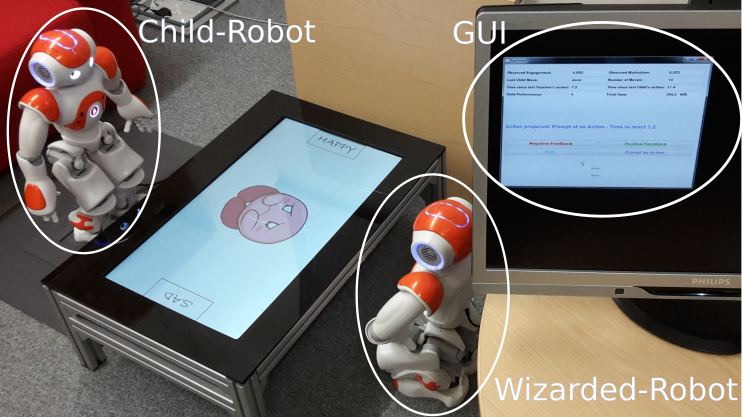
\includegraphics[width=0.65\textwidth]{woz_setup_annotated.png}
	\caption{Setup used for the user study from the perspective of the human supervisor. The \textit{child-robot} (left) stands across the touchscreen (centre-left) from the \textit{wizarded-robot} (centre-right). The supervisor can oversee the actions of the \textit{wizarded-robot} through the GUI and intervene if necessary (right).}
	\label{fig:setup}
\end{figure}
		
\subsection{Child model}

The purpose of the child model is not to realistically model a child (with or without autism), but to provide a means of expressing some of the behaviours we observed in our interactions with children in a repeatable manner.
The child-robot possesses an internal model encompassing an \emph{engagement} level and a \emph{motivation} level, together forming the \textit{state} of the child. 
The engagement represents how often the child-robot will make categorisation moves and the motivation gives the probability of success of the categorisation moves. Bound to the range $[-1, 1]$, these states are influenced by the behaviour of the wizarded-robot, and will asymptotically decay to zero without any actions from the wizarded-robot.
These two states are not directly accessed by either the supervisor or the wizarded-robot, but can be observed through behaviour expressed by the child-robot: low engagement will make the robot look away from the touchscreen, and the speed of the categorisation moves is related to the motivation (to which gaussian noise was added). There is thus incomplete/unreliable information available to both the wizarded-robot and the supervisor, making the task non-trivial.

The influence of the wizarded-robot behaviour on the levels of engagement and motivation are described below (section \ref{sec:wizarded-robot}). In addition to this, if a state is already high and an action from the wizarded-robot further increases it, then there is a chance that this level will sharply decrease, as an analogue of child-robot \textit{frustration}.
When this happens, the child-robot will indicate this frustration verbally (uttering one of eight predefined strings).
The reason this mechanism is required is that it prevents a straightforward engagement and motivation maximisation strategy, thus better approximating the real situation, and requiring a more complex strategy to be employed by the supervisor.

\subsection{Wizarded-robot control}
\label{sec:wizarded-robot}
The wizarded-robot is controlled through a Graphical User Interface (GUI) and has access to multiple variables characterising the state of the interaction. 
The wizarded-robot has a set of four actions, which each have a button in the GUI: 
\begin{itemize}
	\item Prompt an Action: Encourage the child-robot to do an action.
	\item Positive Feedback: Congratulate the child-robot on making a good classification.
	\item Negative Feedback: Supportive feedback for an incorrect classification.
	\item Wait: Do nothing for this action opportunity, wait for the next one.
\end{itemize}

The impact of the action on the child-robot depends on the internal state and the type of the last child-robot move: good, bad, or done (meaning that feedback has already been given for the last move and supplementary feedback is not necessary). 
A prompt always increases the engagement, a wait has no effect on the child-robot's state, and the impact of positive and negative feedback depends on the previous child-robot move.
Congruous feedback (positive feedback for correct moves; negative feedback for incorrect moves) results in an increase in motivation, but incongruous feedback can decrease both the motivation and the engagement of the child-robot.
The supervisor therefore has to use congruous feedback and prompts, whilst being careful not to use them too often, to prevent the child-robot becoming frustrated.
A `good' strategy would keep the engagement and motivation high, leading to an increase in performance of the child-robot in the categorisation task.

Through the GUI, the supervisor has access to \textit{observed states} (noisy estimations of the child-robot state), and information about the interaction history: number of moves, child-robot performance, time since last child-robot and wizarded-robot actions, type of the last child-robot move, and elapsed time.
However the supervisor can not control the wizarded-robot directly, actions can only be executed only at specific times triggered by the wizarded-robot. 
Two seconds after each child-robot action, or if nothing happens in the interaction for five seconds, the wizarded-robot proposes an action to the supervisor by displaying the action's name and a countdown before execution. 
Only after this proposition has been done can the supervisor provide feedback to the wizarded-robot.
If the supervisor does nothing in the following three seconds, the action proposed by the wizarded-robot is executed.
This mechanism allows the supervisor to passively accept a suggestion made by the wizarded-robot or actively make an \emph{intervention} by selecting a different action and forcing the wizarded-robot to execute it.

\subsection{Learning algorithm}

The two robot controllers used for the study were a learning controller and a non-learning random action selection controller.
The learning algorithm used was a Multi-Layer Perceptron, 
%a reviewer asked for more informations about the learning algorithm, should this be added? But it is quite irrelevant for the purpose of the paper...
% with five input nodes: one for the observed motivation, one for the observed engagement and three binary (+1/-1) inputs for the type of the previous move: good, bad, or done. The hidden layer had six nodes and four for the output layer: one for each action. The suggested action was selected applying a Winner-Take-All strategy on the value of the output node and then displayed on the GUI before execution. The network was 
trained with back propagation (five input, six hidden and four output nodes): after each new decision from the supervisor, the network was fully retrained with all the previous state-action pairs and the new one.
%On the other side, the random controller proposed random actions to the supervisor.

\subsection{Participants}

In WoZ scenarios, the wizard is typically a technically competent person with previous experience controlling robots.
As such, to maintain consistency with the target user group, the participants for this study (assuming the role of the supervisor) are taken from a robotics research group.
Ten participants were used (7M/3F, age \textit{M}=29.3, 21 to 44, \textit{SD}=4.8 years).

\subsection{Interaction Protocol}

Each participant experienced both robot controllers, with the order changed between participants to control for any ordering effects.
In \textit{Condition LN} the participants first interact with the learning wizarded-robot, and then with the non-learning one; in \textit{Condition NL} the participants first interact with the non-learning wizarded-robot, and then the learning robot. 
Participants were randomly assigned to one of the two conditions.

The interactions took place on a university campus in a dedicated experiment room.
Two Aldebaran Nao robots were used; one robot had a label indicating that it was the \emph{Child-Robot}. 
The robots face each other with a touchscreen between them, and participants assuming the role of the supervisor sit at a desk to the side of the wizarded-robot, with a screen and a mouse to interact with the wizarded-robot (fig. \ref{fig:setup}).
The participants were able to see the screen and the child-robot.

A document explaining the interaction scenario was provided to participants. After the information had been read, a 30s video presenting the GUI in use was shown to familiarise them with it, without biasing them towards any particular intervention strategy.
The participant then clicked a button to start the first interaction which lasted for 10 minutes.
The experimenter was sat in the room outside of the participants' field of view.
After the end of the first interaction, a post-interaction questionnaire was administered. 
The same protocol was applied in the second part of the experiment with another post-interaction questionnaire following. Finally, a questionnaire asking the participants to explicitly compare the two conditions was administered.

\section{Results}

\section{Discussion}

\section{Summary}

